\FloatBarrier

\begin{figure}[h!]
	\centering
	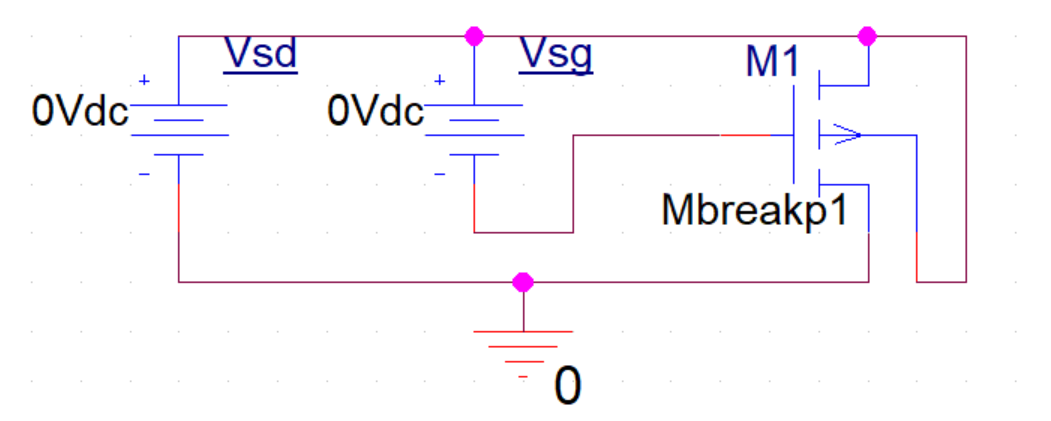
\includegraphics[scale=0.5]{./images/circuit2.PNG}
	\caption{PMOS Circuit}
	\label{fig:circuit2}
\end{figure}

\FloatBarrier

The PMOS transistor has behavior similar to the NMOS, but with a few slight deviations. When the MOS capacitor is charged at a voltage lower than the source, holes are attracted to form the channel. The terminal from which carriers flow shall be called the source. So, for the PMOS, the source terminal should be higher than the drain terminal so that holes can flow from high to low potential from the source. Therefore, current flows into the drain, unlike in an NMOS transistor, where the current flows away from the drain. So, the NMOS current plot should be flipped over the x-axis for the PMOS since the current is negative.

\FloatBarrier

\begin{figure}[h!]
	\centering
	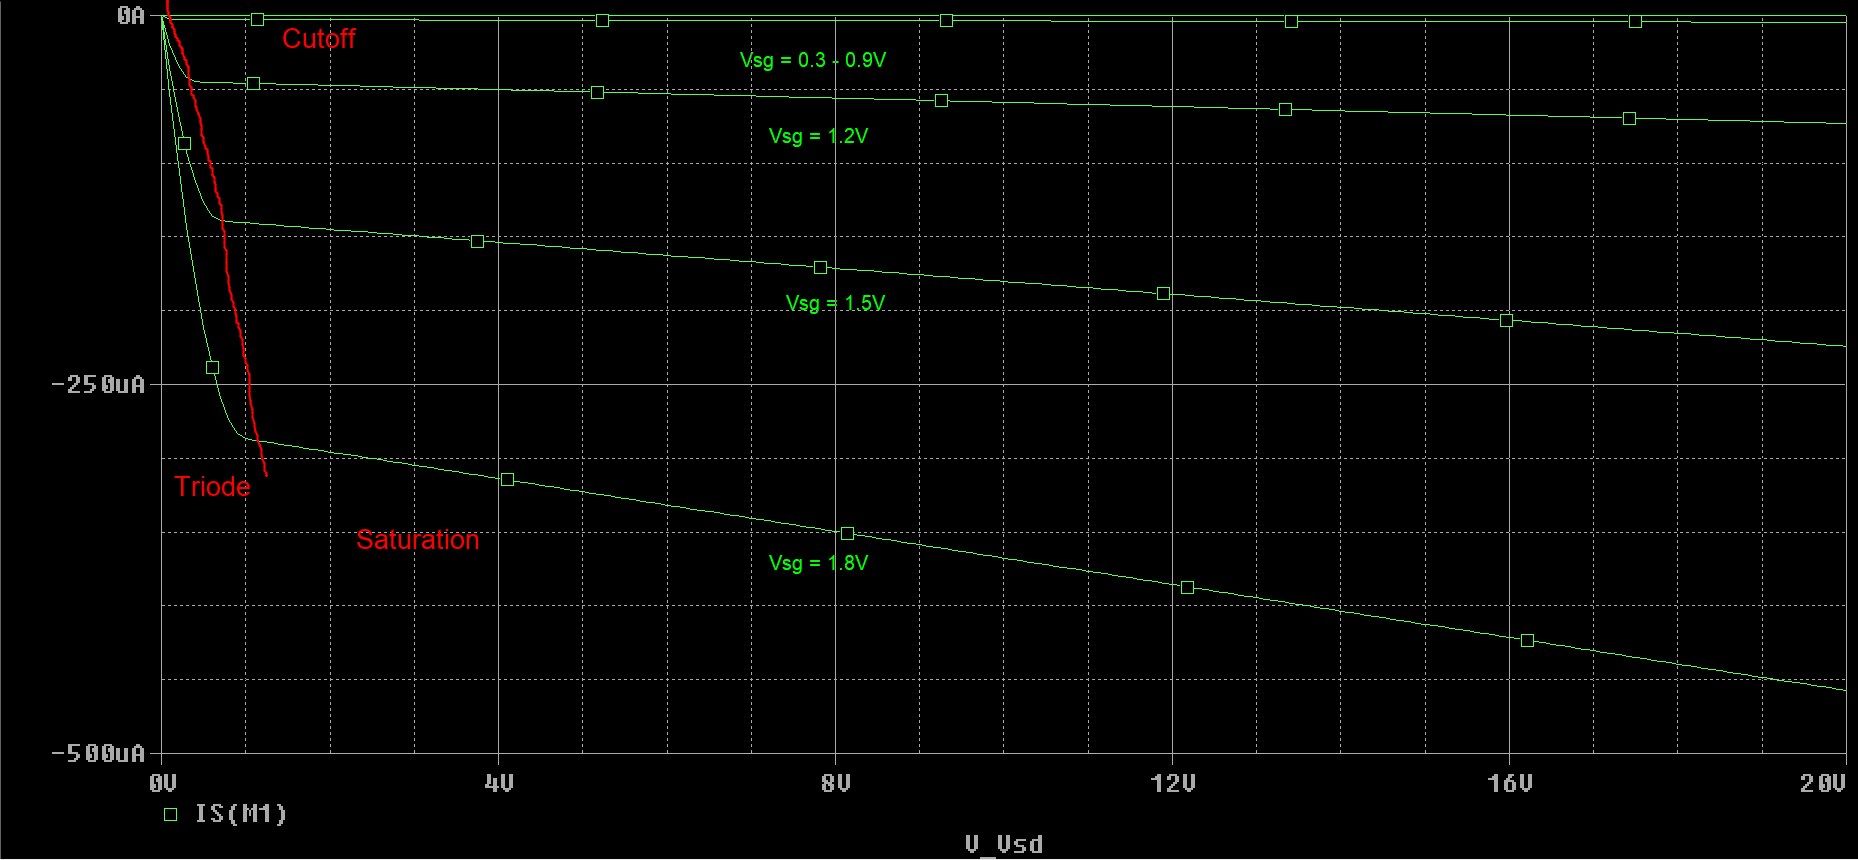
\includegraphics[scale=0.25]{./images/circuit2_vsd_sweep.PNG}
	\caption{PMOS $i_{D}$ versus $V_{SD}$}
	\label{fig:circuit2_vsd_sweep}
\end{figure}

\FloatBarrier

If only the magnitude is observed, the plots should turn out to be the same. The voltages applied to the transistor are essentially the same, with source and drain terminals flipped, giving rise to the factor of $-1$ difference between the NMOS and PMOS current plots. For the SPICE models used, the PMOS has a process transconductance parameter $k_p \approx \frac{k_n}{2}$. The PMOS's process transconductance parameter is given by:

\begin{equation}
	\label{eq:pmos_trans}
	k_p' = \mu _{p} C_{ox}
\end{equation}

The NMOS's parameter is:

\begin{equation}
	\label{eq:nmos_trans}
	k_n' = \mu _{n} C_{ox}
\end{equation}

Here, $C_{ox}$ is the oxide capacitance density per area, $\mu _{n}$ is the electron mobility, and $\mu _{p}$ is the hole mobility. $k_p'$ is about half the magnitude of $k_n'$ because the hole mobility $\mu _{p}$ is about half the magnitude of $\mu _{n}$.

The drain currents in transistors depend on the MOSFET transconductance parameter, which for a PMOS is given by:

\begin{equation}
	\label{eq:pmos_fettrans}
	k_p = k_p' \frac{W}{L}
\end{equation}

% TODO Mention the actual values from the model of kp and kp'

$W$ is the transistor's channel width, and $L$ is the channel length. Making the width $W$ twice the width of the corresponding NMOS model compensates for the lower process transconductance parameter. Thus, the PMOS's $|i_D|$ curve should be the same as the NMOS's. The factor of $-1$ difference for the $i_D$ plots should be the only difference between the two.

\FloatBarrier

\begin{figure}[h!]
	\centering
	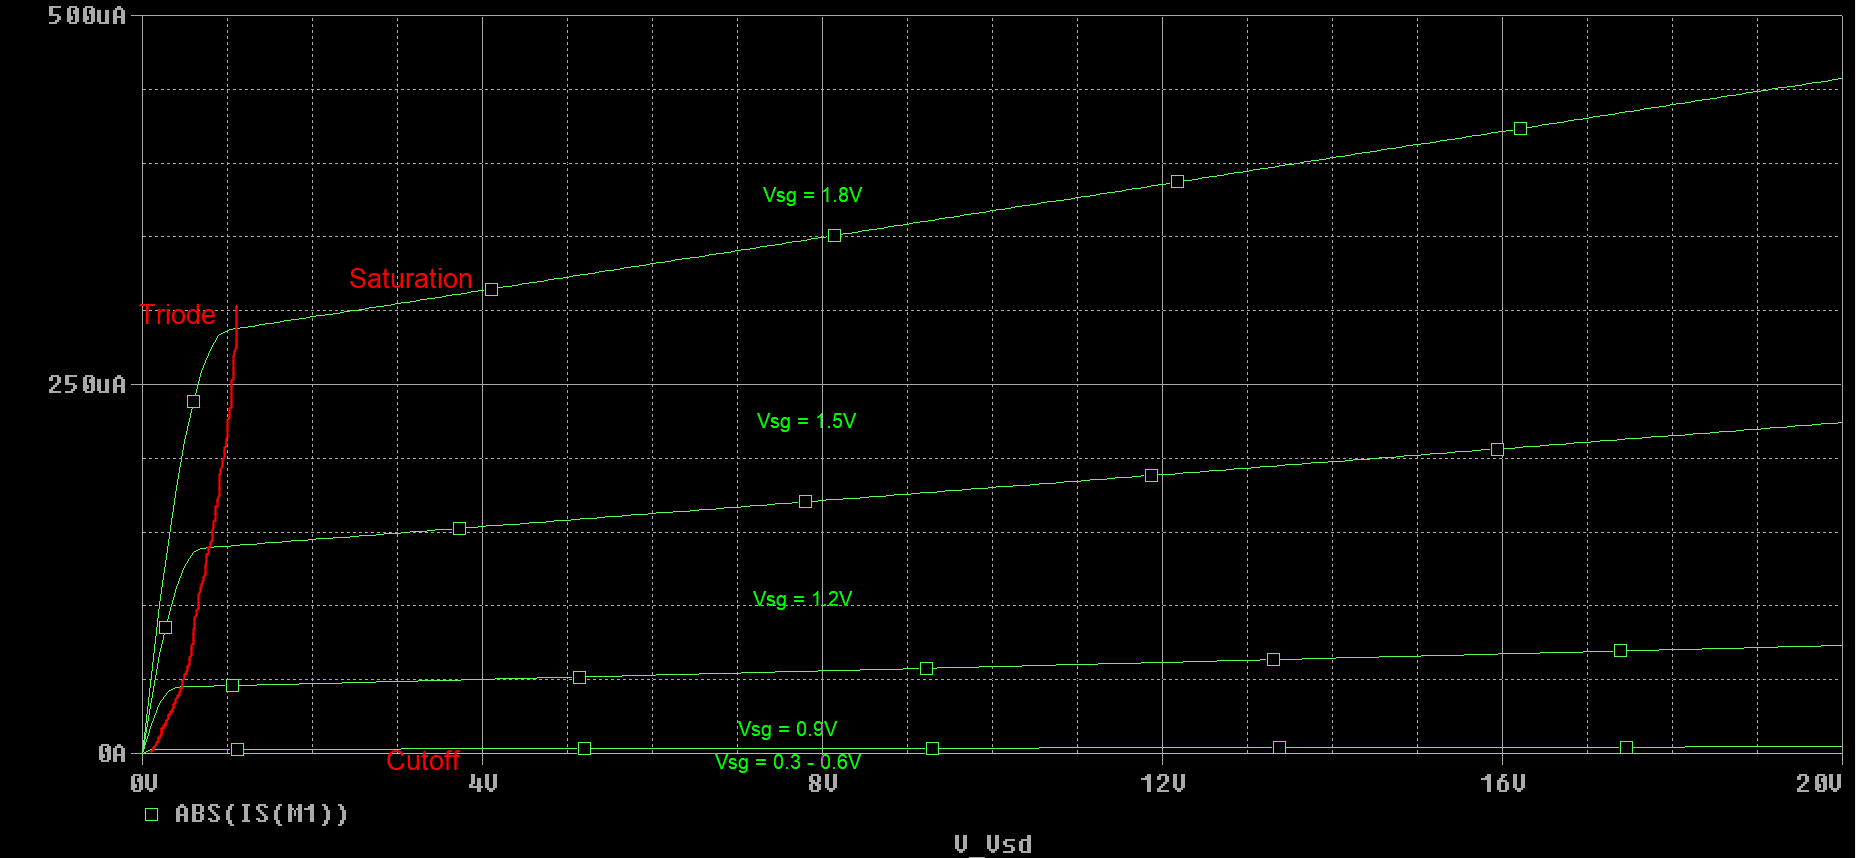
\includegraphics[scale=0.25]{./images/circuit2_vsd_sweep_abs.PNG}
	\caption{PMOS $|i_D|$ vs $V_{SD}$}
	\label{fig:circuit2_vsd_sweep_abs}
\end{figure}

\FloatBarrier

%id vs vds curves

When sweeping $V_{SD}$, the mechanics of the PMOS transistor are nearly identical besides the fact that holes are the charge carrier. As a result, the drain current differs by a factor of $-1$. The $|i_D|$ curve is essentially the same as for the NMOS for the same reasons as above. \\

The same logic applies to the $i_{D}$ versus $V_{SG}$ curves. The difference is in the factor of $-1$.

\FloatBarrier

\begin{figure}[h!]
	\centering
	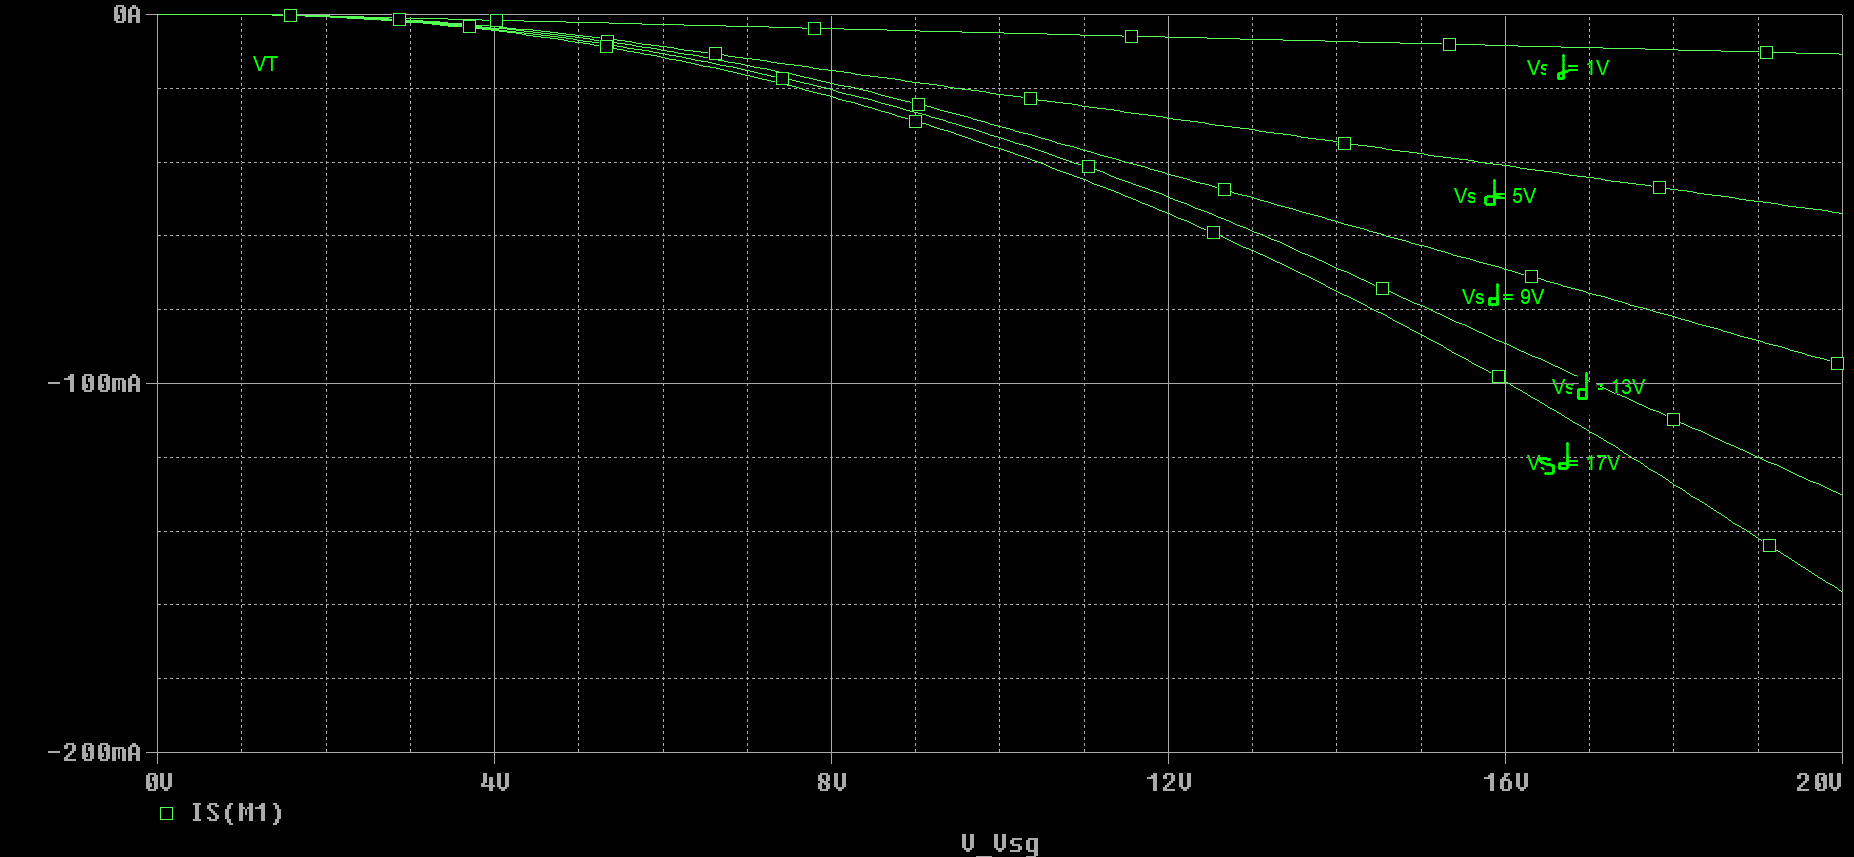
\includegraphics[scale=0.25]{./images/id_vs_vsg.PNG}
	\caption{PMOS $i_D$ vs $V_{SG}$}
	\label{fig:id_vs_vsg}
\end{figure}

\FloatBarrier

\FloatBarrier

\begin{figure}[h!]
	\centering
	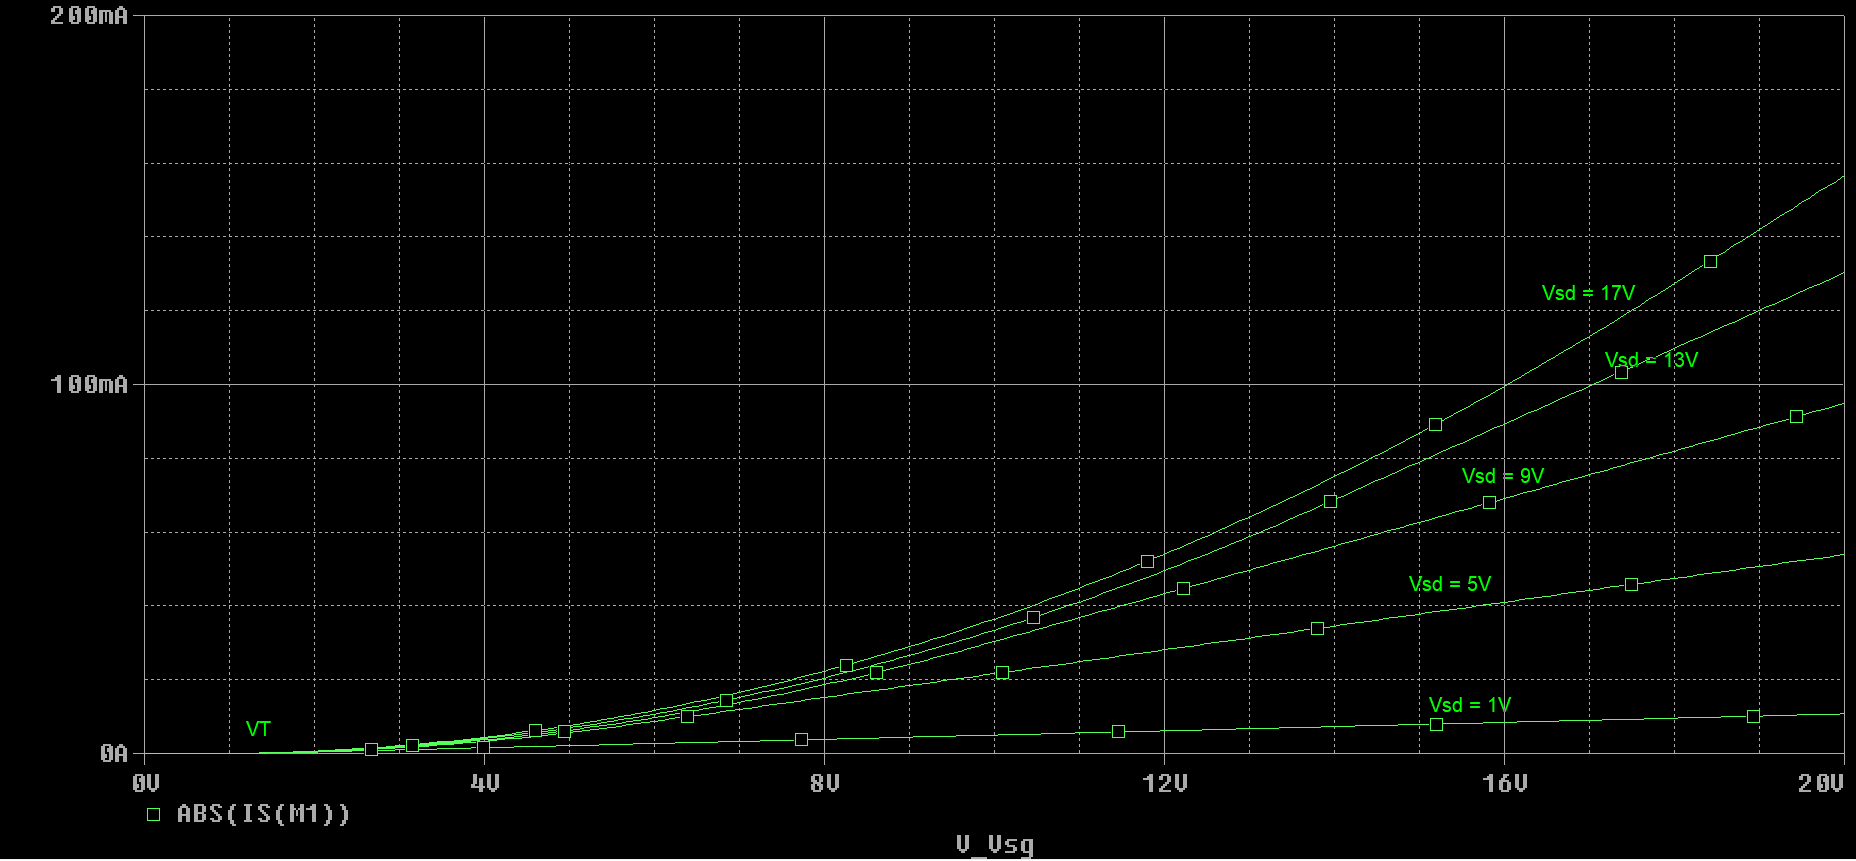
\includegraphics[scale=0.5]{./images/id_vs_vsg_abs.PNG}
	\caption{PMOS $|i_D|$ vs $V_{SG}$}
	\label{fig:id_vs_vsg_abs}
\end{figure}

\FloatBarrier
